% !TEX root = ../main.tex
\pagebreak[0]
\section{\emph{Endpoint} and \emph{crossing} configurations}\label{sec:endpoint-and-crossing-configurations}

\begin{figure}[htbp]
\centering
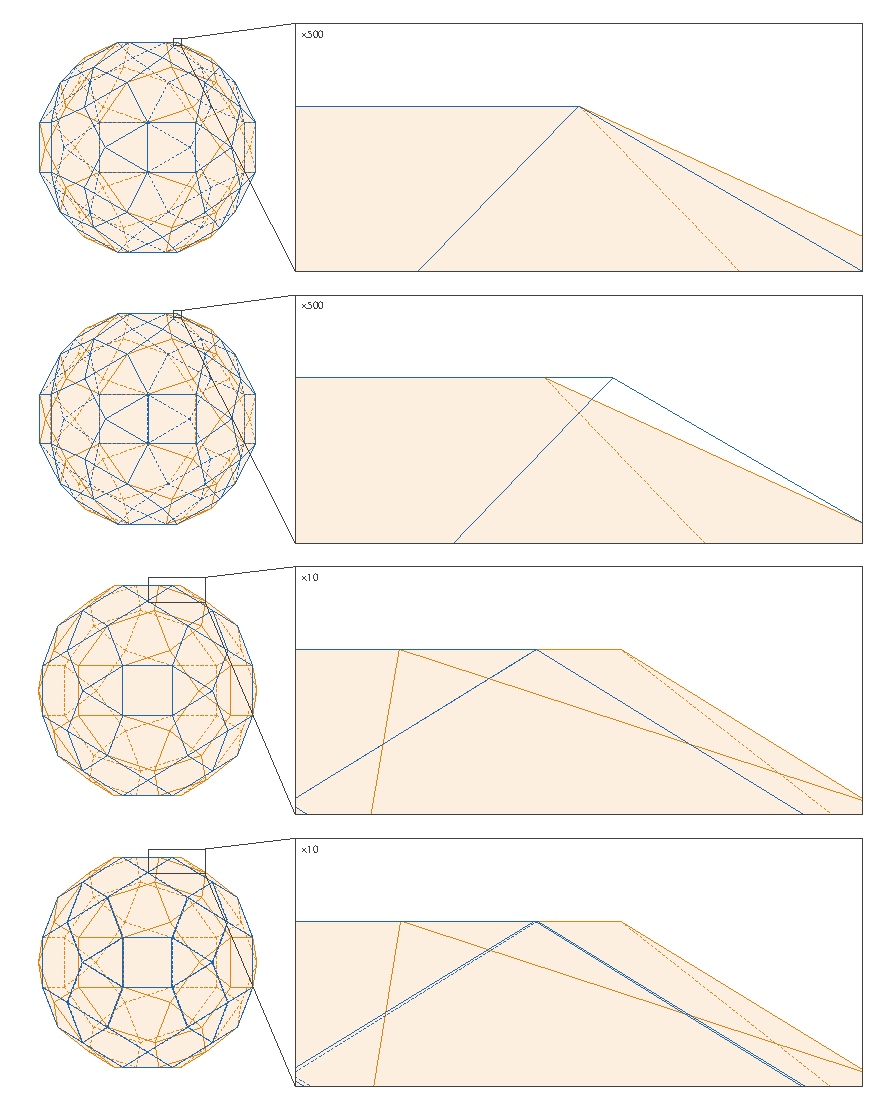
\includegraphics[width=\linewidth]{figures/endpoint-crossing}
\caption{Configurations in the plane $\Pi_1$, enlarged at the right ends of the two top edges as in \cref{fig:arc-examples}, $500$ times for the first two and $10$ times for the last two; the \fc{Hole}{hole (orange)} and the \fc{Plug}{plug (blue)} as in \cref{fig:global-examples}. First: the endpoint $e=e_*$, where the ends of the two top edges coincide. Second: $e=e_*+1/256$ on the continuation of the first arc, where the plug's top edge is longer than the hole's and its corner protrudes, a poke configuration. Third: the crossing $e=0$. Fourth: the configuration $e=1/200$, $\theta=-1/200$ of the second arc, which lies outside $D$.}
\label{fig:endpoint-crossing-examples}
\end{figure}

At the two ends of the first arc, the rate of outward motion off the arc
plane shrinks to zero, as it did at the square and pentagon
configurations. The remedy is the same: point zooms that divide out two
distances, the distance along the arc from the special configuration and
the displacement off the arc measured relative to it. The crossing needs
one further idea, because the second arc passes through it.

Both covers use the arc coordinates \cref{eq:arc-coordinates} of one plane
$\Pi_\sigma$ and come in two copies, one for each sign $\sigma$. Their base
coordinate is $e$ measured from the special configuration, and their offset
coordinates are those of the arc covers, with $v$ weighted.

\subsection{Eliminating the \emph{endpoint} configuration}\label{subsec:eliminating-the-endpoint-configuration}

At the endpoint $e=e_*$, the first arc ends: beyond it, the configurations
of the plane poke. Around it we use a point zoom cover as in
\cref{sec:square-and-pentagon-configurations}, with base coordinate
$e-e_*$ and $\Sigma=[-1,1]$, offset coordinates $(v/2,\theta,\zeta_1,\zeta_3)$
with $\Phi=[0,1]\times{[-1,1]}^3$, and ratio $\rho_0=1$. The base radius is
$1/16$ on the face $e<e_*$ and $1/32$ on the face $e>e_*$, and the offset
radius is $\delta_{\max}=1/32$. The two base faces and seven offset faces
give 14 zooms in family A and seven in family B. The covered set consists
of the configurations with
\[
  -\frac1{16}\le e-e_*\le\frac1{32},\qquad 0\le v\le\frac1{16},\qquad
  |\theta|,|\zeta_1|,|\zeta_3|\le\frac1{32}.
\]
The no-fit set of the zooms is the plane $\Pi_\sigma$, by
\cref{lem:arc-planes-contain-no-fit}.
As at the square configuration, some directions of displacement move no
projected vertex outward at first order at the endpoint itself, and the
cells there use two kinds of witnesses: one whose limit after division
contains the base coordinate, and a radial one.

\begin{proposition}[The endpoint neighbourhoods]\label{prop:endpoint-neighbourhoods}
  For each $\sigma\in\{-1,1\}$, no configuration of $D$ in the covered set
  above is a fit.
\end{proposition}
\begin{proof}
  As for \cref{prop:arc-neighbourhoods}, with \cref{lem:point-coverage}
  in place of \cref{lem:tube-coverage}.
\end{proof}

\subsection{Eliminating the \emph{crossing} configuration}\label{subsec:eliminating-the-crossing-configuration}

At the crossing $e=0$, the second arc $\theta=-e$ meets the first. The point
zoom cover around it has base coordinate $e$ with $\Sigma=[-1,1]$, offset
coordinates $(4v/5,\theta,\zeta_1,\zeta_3)$ with $\Phi=[0,1]\times{[-1,1]}^3$,
radii $\mu_{\max}=\delta_{\max}=1/16$ and ratio $\rho_0=5/4$: 14 zooms in
family A and seven in family B, with the covered set
\[
  |e|\le\frac1{16},\qquad 0\le v\le\frac5{64},\qquad
  |\theta|,|\zeta_1|,|\zeta_3|\le\frac1{16}.
\]
The distance coordinates of these zooms vanish only on the segment
$\theta=0$, $|e|\le1/16$ of $\Pi_\sigma$, which contains the first arc near
the crossing; the no-fit set of the zooms is $\Pi_\sigma$, by
\cref{lem:arc-planes-contain-no-fit}. The second arc, however, is also a
family of touch configurations, and it runs through the domain of one
zoom. In the family A zoom on the base face
$e=\mu>0$ and the offset face $\theta=-1$, the second arc is the set where
$\rho=1$ and the other offset coordinates vanish. No gap polynomial is
positive at a touch configuration. The fold inequality is violated on the
second arc for $e>0$ (\cref{sec:arc-configurations}), but at the crossing its
polynomial has first-order terms in $v$, $\zeta_1$ and $\zeta_3$: in this zoom
it is divisible only by $\mu$, and its quotient at $\mu=0$ is $\rho$ times a
linear form in the off-plane offsets, which vanishes on the second arc. So
no cell containing the end $\mu=0$ of the second arc can pass the test. Whatever the ratio, the second arc meets some zoom domain;
with $\rho_0=5/4>1$ it lies inside family A only, away from the boundary
$\rho=\rho_0$ between the two families, and only cells of family A need
the following treatment.

\paragraph{Handing cells over.}
The cells of family A along the second arc are covered by other zooms,
built in the same way around the second arc instead of the first. The
\emph{sheared} offset $\theta'=\theta+e$ measures the displacement from the
second arc. The sheared zooms $\mathcal A'_{G,F}$, for the base face $G$
with $e>0$ and every offset face $F$, are the zooms of family A with
$\theta'$ in place of $\theta$ and the ratio $\rho'\in[0,\rho_0']$,
$\rho_0'=1/4$. Their distance coordinates vanish only on the second arc,
which lies in the no-fit plane $\Pi_\sigma$. A cell of family A whose
configurations, measured from the second arc, stay within the domains of
the sheared zooms needs no witness of its own: it is \emph{handed over},
and the checked cells of the sheared zooms take its place.

To state this precisely, let $\mathcal A_{G,F}$ be a zoom of family A on
the base face $G$ with $e>0$, so that $e=\mu$, and write
\[
  \mathbf o(\mathbf y)=\rho\widehat{\mathbf f}+(0,1,0,0)
\]
for the offset measured from the second arc in units of $\mu$: the shear
adds $e=\mu$ to the second offset coordinate $\theta$.

\begin{lemma}[Hand-over]\label{lem:hand-over}
  Let $C$ be a cell of a zoom $\mathcal A_{G,F}$ of family A, on the base
  face $G$ with $e>0$, such that $\mathbf o(\mathbf y)\in\rho_0'\Phi$ for every
  $\mathbf y\in C$. Then every configuration in the image of $C$ lies in the
  no-fit set or is the image of a point in the domain of one of the sheared
  zooms $\mathcal A'_{G,F'}$.
\end{lemma}
\begin{proof}
  At $\mathbf y\in C$, the base coordinate is $\mu$ and the sheared offset
  is $\mu\,\mathbf o(\mathbf y)$. If $\mathbf o(\mathbf y)=\mathbf0$, the
  configuration lies on the second arc, in the no-fit set. Otherwise
  $\rho'=\lVert\mathbf o(\mathbf y)\rVert_\infty\in(0,\rho_0']$, and
  $\widehat{\mathbf f}'=\mathbf o(\mathbf y)/\rho'$ lies on a face $F'$ of $\Phi$,
  giving a point of the domain of $\mathcal A'_{G,F'}$ with the same
  configuration.
\end{proof}

The hypothesis is checked exactly for each handed-over cell: each
coordinate of $\mathbf o$ is the product of two zoom coordinates, plus a
constant for the second, so its exact range over the cell follows from
interval products. Cells are handed over only from family A to the sheared
family, never back. The cover for $\sigma=1$ hands 34 cells over, and the
cover for $\sigma=-1$ hands over 14 (\cref{fig:crossing-plane}).

\begin{figure}[htbp]
\centering
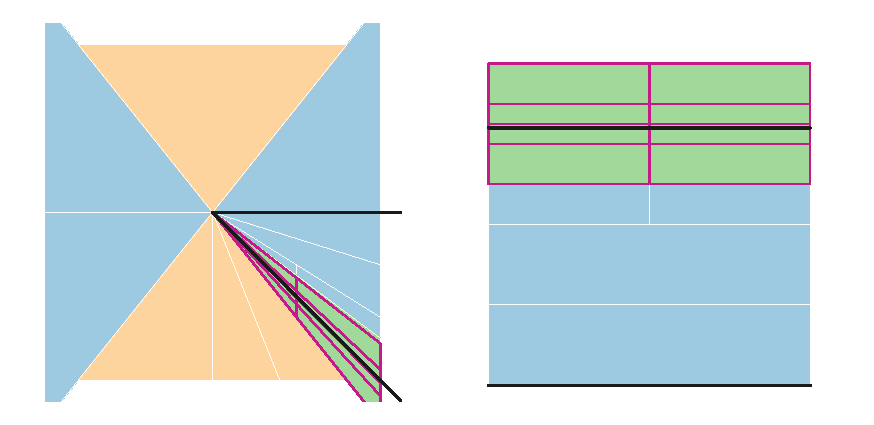
\includegraphics[width=\linewidth]{figures/crossing-plane}
\caption{The crossing cover of $\Pi_1$ where it meets the plane itself ($v=\zeta_1=\zeta_3=0$). Left: in the coordinates $(e,\theta)$, both in $[-9/128,9/128]$, the cells of \fc{Global}{family A (light blue}; $|\theta|\le\tfrac54|e|$, cut by rays of constant ratio), of \fc{FamilyB}{family B (light orange}; $|e|\le\tfrac45|\theta|$) and of \fc{Sheared}{the sheared zooms around the second arc (green)}; \fc{Crossing}{the cells of family A handed over to the sheared zooms are outlined in magenta}, and the first arc $\theta=0$ and the second arc $\theta=-e$ are black. Right: the family A zoom on the base face $e=\mu>0$ and the offset face $\theta=-1$, in its own coordinates ($20\mu\in[0,5/4]$ horizontally, $\rho\in[0,5/4]$ vertically), in which the first arc is $\rho=0$ and the second arc $\rho=1$ (black): \fc{Global}{its cells in the plane (light blue)} and, along $\rho=1$, \fc{Sheared}{the cells it hands over (green,} \fc{Crossing}{outlined in magenta}). Most of the refinement of this cover happens in $v$, $\zeta_1$ and $\zeta_3$, so few cells meet the plane.}
\label{fig:crossing-plane}
\end{figure}

\begin{proposition}[The crossing neighbourhoods]\label{prop:crossing-neighbourhoods}
  For each $\sigma\in\{-1,1\}$, no configuration of $D$ in the covered set
  above is a fit.
\end{proposition}
\begin{proof}
  By \cref{lem:point-coverage}, a configuration of the covered set lies in
  the no-fit set $\Pi_\sigma$, in a checked cell with a witness, or in a
  handed-over cell.
  The first two cases are as for \cref{prop:arc-neighbourhoods}. In the
  third, \cref{lem:hand-over} places the configuration on the second arc
  or in the domain of a sheared zoom, whose cells are checked by
  \cref{lem:zoom-lemma}.
\end{proof}

\subsection{The arcs together}\label{subsec:the-arcs-together}

The covers along the first arc overlap: the arc cover and the crossing
cover share $3/64\le e\le1/16$, and the arc cover and the endpoint cover
share $e_*-1/16\le e\le3/16$. Every configuration of the first arc with
$0\le e\le e_*$ therefore lies in the interior, relative to $B_0$, of the
covered set of one cover, and so in the collection's range. The second arc
lies outside $D$ for $e>0$ and meets the crossing cover at $e=0$. Together
with \cref{prop:aligned-neighbourhood}, the collection's range contains a
neighbourhood of every touch configuration of $D$ that the subdivision
revealed. That the collection eliminates every box is confirmed by the
search itself, in \cref{sec:generating-and-verifying-the-certificate}.
